\documentclass[12pt, twoside]{article}
\usepackage[letterpaper, margin=1in, headsep=0.2in]{geometry}
\setlength{\headheight}{0.6in}
%\usepackage[english]{babel}
\usepackage[utf8]{inputenc}
\usepackage{microtype}
\usepackage{amsmath}
\usepackage{amssymb}
%\usepackage{amsfonts}
\usepackage{siunitx} %units in math. eg 20\milli\meter
\usepackage{yhmath} % for arcs, overparenth command
\usepackage{tikz} %graphics
\usetikzlibrary{quotes, angles}
\usepackage{graphicx} %consider setting \graphicspath{{images/}}
\usepackage{parskip} %no paragraph indent
\usepackage{enumitem}
\usepackage{multicol}
\usepackage{venndiagram}

\usepackage{fancyhdr}
\pagestyle{fancy}
\fancyhf{}
\renewcommand{\headrulewidth}{0pt} % disable the underline of the header
\raggedbottom
\hfuzz=2mm %suppresses overfull box warnings

\usepackage{hyperref}

\fancyhead[LE]{\thepage}
\fancyhead[RO]{\thepage \\ Name: \hspace{4cm} \,\\}
\fancyhead[LO]{BECA / Dr. Huson / Geometry\\*  Unit 9: Dilation \\* 17 January 2022}

\begin{document}

\subsubsection*{9.1 Classwork: Dilation \hfill CCSS.HSG.SRT.B.5}
\begin{enumerate}
    \item Do Now: Plot and label the triangle $A'B'C'$. $A'(0,0)$, $B'(8,0)$, $C'(8,4)$.\\
    Make a list of comparisons of the two triangles: their sides' lengths, location, their angles, orientation, area and perimeter. \\
      \begin{tikzpicture}[scale=.7]
        \draw [help lines] (-1,-2) grid (9,6);
        \draw [thick, ->] (-1.2,0) -- (9.4,0) node [below right] {$x$};
        \draw [thick, ->] (0,-2.2)--(0,6.4) node [left] {$y$};
        \draw [thick] (0,0)node[below right]{$A$}--
         (4,0)node[below]{$B$}--
           (4,2)node[above left]{$C$}--cycle;
      \end{tikzpicture}
     \vspace{3cm}
  
\begin{multicols}{2}
[\item Find the missing angle measures. Are $\triangle CAT$ and $\triangle DOG$ congruent?] \vspace{0.5cm}
    \begin{tikzpicture}[scale=0.9]
      \coordinate [label=above left:$C$](A) at (95:2);
      \coordinate [label=below:$A$](B) at (0, 0);
      \coordinate [label=right:$T$](C) at (-10:3.5);
      \draw [thick] (A)--(B)--(C)--cycle;
      \draw [thick, xshift=3cm, yshift=1.5cm, scale=1.5] (95:2) node[above]{$D$}--
      (0,0) node[below]{$O$}--
      (-10:3.5) node[right]{$G$}--cycle;
    \end{tikzpicture}\\
    \begin{enumerate}
      \item $m\angle C =45^\circ$, $m\angle A =105^\circ$\\[0.25cm]
      .\hspace{1cm} $m\angle T =$ \rule{2cm}{0.15mm}
      \item $m\angle G =30^\circ$, $m\angle O =105^\circ$\\[0.5cm]
      .\hspace{1cm} $m\angle D =$ \rule{2cm}{0.15mm}
    \end{enumerate}
  \end{multicols}  \vspace{1cm}
      
\item This is the symbol for similar triangles: $\triangle ABC \sim \triangle DEF$. Write down two definitions of similar triangles.
  
\newpage
\item \begin{enumerate}
  \item Graph and label $\triangle ABC$ with $A(0,0)$, $B(3,2)$, and $C(3,0)$.
  \begin{center}
    \begin{tikzpicture}%[scale=.635]
      \draw [help lines] (0,0) grid (10,6);
      \draw [thick, ->] (0,0) -- (10.4,0) node [below right] {$x$};
      \draw [thick, ->] (0,0)--(0,6.4) node [left] {$y$};
    \end{tikzpicture}
  \end{center}
  \item Dilate or stretch the triangle by a factor of $k=3$ centered at the origin.\\ $\triangle ABC \rightarrow \triangle A'B'C'$
  \item Find each ratio or fraction. \\[0.5cm]
    $\displaystyle \frac{A'C'}{AC}=$ \hfill
    $\displaystyle \frac{B'C'}{BC}=$ \hfill
    $\displaystyle \frac{A'B'}{AB}=$ \hspace{2cm}
\vspace{1cm}
\end{enumerate}
\item Triangle $ABC$ is dilated with a scale factor of $k=\frac{5}{3}$ centered at $A$, yielding $\triangle ADE$, as shown. Given $AB=9$, $BC=12$, and $AC=15$. \\[0.25cm] Find $AD$, $AE$, and $DE$. \vspace{0.5cm}
   \begin{center}
       \begin{tikzpicture}[scale=0.4]
         \draw [thick]
         (0,0)node[left]{$B$}--
         (8,0)node[above right]{$C$}--
         (2,6)node[left]{$A$}--cycle;
         \draw [thick]
         (0,0)--
         (-1,-3)node[left]{$D$}--
         (11,-3)node[above right]{$E$}--(8,0);
         \node at (4,0)[below]{$12$};
         \node at (5.3, 3)[right]{$15$};
         \node at (0.3, 2.8)[above]{$9$};
       \end{tikzpicture}
     \end{center}

\newpage
Definition of \emph{similar} triangles: Triangles that have the same shape, but not necessarily the same size, are similar. Their corresponding angles are congruent and their corresponding sides are proportional. \\[1cm]
Dilation definition of similarity: Two figures are similar if one or more rigid motions and a dilation will carry one figure onto the other.

\item Vocabulary: A dilation stretches or shrinks. It has a \emph{center} and a \emph{scale factor, k}. \\[0.5cm]
A dilation centered at $A$ with scale factor $k=2$ maps $\triangle ABC \rightarrow \triangle ADE$. Given the sides of the preimage, $AC = 4$, $BC = 3$, $AB = 5$. \\[0.5cm]
$DE = 6$, how long are $AD$ and $AE$?
    \begin{flushright}
      \begin{tikzpicture}[scale=0.8]
        \draw [-, thick] (0,0)--
        (8,0) node[below]{$E$}--
        (8,6) node[above left]{$D$}--cycle;
        \draw [thick] (4,0)--(4,3);
        \draw [fill] (0,0) circle [radius=0.1] node[below] {$A$};
        \node at (4,0) [below]{$C$};
        \node at (4,3) [above left]{$B$};
        \node at (2, 0) [below]{$4$};
        \node at (2, 2) [above]{$5$};
        \node at (8, 3) [right]{$6$};
        \node at (4, 1.5) [right]{$3$};
      \end{tikzpicture}
    \end{flushright}

\item Dilate $\triangle ABC \rightarrow \triangle A'B'C'$ by a factor of $k=2$ centered at the origin, $(x,y) \rightarrow (2x, 2y)$. Plot and label the image on the axes. Make a table of the vertices and their coordinates.
\begin{flushright}
    \begin{tikzpicture}[scale=1]
    \draw [help lines] (-1,-2) grid (5,7);
    \draw [thick, <->] (-1.4,0) -- (5.4,0) node [right] {$x$};
    \draw [thick, <->] (0,-2.4)--(0,7.4) node [above] {$y$};  
    \draw [thick]
      (0,0) node[below left] {$A$}--
      (2,3) node[above left] {$B$}--
      (2,0) node[below] {$C$}--cycle;  
  \end{tikzpicture}
\end{flushright}

\item Dilate $\triangle ABC \rightarrow \triangle A'B'C'$ by a factor of $k=3$ centered at the origin, $(x,y) \rightarrow (3x, 3y)$. Plot and label the image on the axes. Make a table of the vertices and their coordinates.
\begin{flushright}
    \begin{tikzpicture}[scale=1]
    \draw [help lines] (-1,-3) grid (7,7);
    \draw [thick, <->] (-1.4,0) -- (7.4,0) node [right] {$x$};
    \draw [thick, <->] (0,-3.4)--(0,7.4) node [above] {$y$};  
    \draw [thick]
      (0,0) node[below left] {$A$}--
      (2,2) node[above left] {$B$}--
      (1,-1) node[below left] {$C$}--cycle;  
  \end{tikzpicture}
\end{flushright}
    

\item A dilation centered at $A$ with scale factor $k=2$ maps $\triangle ABC \rightarrow \triangle ADE$. Given the sides of the preimage, $AC = 8$, $BC = 6$, $AB = 10$. \\[0.5cm]
$DE = 12$, how long are $AD$ and $AE$?
    \begin{flushright}
      \begin{tikzpicture}[scale=0.8]
        \draw [-, thick] (0,0)--
        (8,0) node[below]{$E$}--
        (8,6) node[above left]{$D$}--cycle;
        \draw [thick] (4,0)--(4,3);
        \draw [fill] (0,0) circle [radius=0.1] node[below] {$A$};
        \node at (4,0) [below]{$C$};
        \node at (4,3) [above left]{$B$};
        \node at (2, 0) [below]{$8$};
        \node at (2, 2) [above]{$10$};
        \node at (8, 3) [right]{$12$};
        \node at (4, 1.5) [right]{$6$};
      \end{tikzpicture}
    \end{flushright}

\item Dilate $\triangle ABC \rightarrow \triangle A'B'C'$ by a factor of $k=1.5$ centered at the origin, $(x,y) \rightarrow (1.5x, 1.5y)$. Plot and label the image on the axes. Make a table of the vertices and their coordinates.
\begin{flushright}
    \begin{tikzpicture}[scale=1]
    \draw [help lines] (-1,-2) grid (5,7);
    \draw [thick, <->] (-1.4,0) -- (5.4,0) node [right] {$x$};
    \draw [thick, <->] (0,-2.4)--(0,7.4) node [above] {$y$};  
    \draw [thick]
      (0,0) node[below left] {$A$}--
      (2,4) node[above left] {$B$}--
      (2,0) node[below] {$C$}--cycle;  
  \end{tikzpicture}
\end{flushright}

\item A transformation is performed on a parallelogram, $BECA \rightarrow B'E'C'A'$, as shown in the diagram. \\[0.5cm]
Fully characterize the transformation. (hint: Translations must include both $x$ and $y$ directions and magnitudes. Dilations must specify the center and scale factor.)
\begin{flushright}
    \begin{tikzpicture}[scale=1]
    \draw [help lines] (-1,-3) grid (7,7);
    \draw [thick, <->] (-1.4,0) -- (7.4,0) node [right] {$x$};
    \draw [thick, <->] (0,-3.4)--(0,7.4) node [above] {$y$};  
    \draw [thick]
      (0,0) node[below left] {$B$}--
      (1,2) node[above left] {$E$}--
      (3,2) node[above left] {$C$}--
      (2,0) node[below left] {$A$}--cycle;
    \draw [thick]
      (0,0) node[below right] {$B'$}--
      (2,4) node[above right] {$E'$}--
      (6,4) node[above right] {$C'$}--
      (4,0) node[below right] {$A'$}--cycle;
  \end{tikzpicture}
\end{flushright}

\item Dilate $\triangle ABC \rightarrow \triangle A'B'C'$ by a factor of $k=3$ centered at the origin, $(x,y) \rightarrow (3x, 3y)$. Plot and label the image on the axes. Make a table of the vertices and their coordinates.
\begin{flushright}
    \begin{tikzpicture}[scale=1]
    \draw [help lines] (-1,-3) grid (7,7);
    \draw [thick, <->] (-1.4,0) -- (7.4,0) node [right] {$x$};
    \draw [thick, <->] (0,-3.4)--(0,7.4) node [above] {$y$};  
    \draw [thick]
      (0,0) node[below left] {$A$}--
      (2,1) node[above left] {$B$}--
      (1,-1) node[below left] {$C$}--cycle;  
  \end{tikzpicture}
\end{flushright}


\item A dilation centered at $A$ with scale factor $k=2$ maps $\triangle ABC \rightarrow \triangle ADE$. Given the sides of the preimage, $AC = 10$, $BC = 7$, $AB = 12$. \\[0.5cm]
  $DE = 14$, how long are $AD$ and $AE$?
      \begin{flushright}
        \begin{tikzpicture}[scale=0.8]
          \draw [-, thick] (0,0)--
          (8,0) node[below]{$E$}--
          (8,6) node[above left]{$D$}--cycle;
          \draw [thick] (4,0)--(4,3);
          \draw [fill] (0,0) circle [radius=0.1] node[below] {$A$};
          \node at (4,0) [below]{$C$};
          \node at (4,3) [above left]{$B$};
          \node at (2, 0) [below]{$10$};
          \node at (2, 2) [above]{$12$};
          \node at (8, 3) [right]{$14$};
          \node at (4, 1.5) [right]{$7$};
        \end{tikzpicture}
      \end{flushright}

\item Dilate $\triangle ABC \rightarrow \triangle A'B'C'$ by a factor of $k=1.5$ centered at the origin,\\
$(x,y) \rightarrow (1.5x, 1.5y)$. Plot and label the image on the axes. Make a table of the vertices and their coordinates.
\begin{flushright}
    \begin{tikzpicture}[scale=0.8]
    \draw [help lines] (-1,-2) grid (9,9);
    \draw [thick, <->] (-1.4,0) -- (9.4,0) node [right] {$x$};
    \draw [thick, <->] (0,-2.4)--(0,9.4) node [above] {$y$};  
    \draw [thick]
      (0,0) node[below left] {$A$}--
      (2,4) node[above left] {$B$}--
      (4,0) node[below] {$C$}--cycle;  
  \end{tikzpicture}
\end{flushright}

\item A transformation is performed on a parallelogram, $MATH \rightarrow M'A'T'H'$, as shown in the diagram. \\[0.5cm]
What is the transformation? (Hint: Is it a translation, reflection, rotation, or dilation? What is its center? What is the scale factor, $k$?)
\begin{flushright}
    \begin{tikzpicture}[scale=0.7]
    \draw [help lines] (-1,-3) grid (10,7);
    \draw [thick, <->] (-1.4,0) -- (10.4,0) node [right] {$x$};
    \draw [thick, <->] (0,-3.4)--(0,7.4) node [above] {$y$};  
    \draw [thick]
      (0,0) node[below left] {$M$}--
      (1,2) node[above left] {$A$}--
      (3,2) node[above left] {$T$}--
      (2,0) node[below right] {$H$}--cycle;
    \draw [thick]
      (0,0) node[below right] {$M'$}--
      (3,6) node[above right] {$A'$}--
      (9,6) node[above right] {$T'$}--
      (6,0) node[below right] {$H'$}--cycle;
  \end{tikzpicture}
\end{flushright}

\item Dilate $\triangle ABC \rightarrow \triangle A'B'C'$ by a factor of $k=2.5$ centered at the origin, \\
$(x,y) \rightarrow (2.5x, 2.5y)$. Plot and label the image on the axes. (table optional)
\begin{flushright}
    \begin{tikzpicture}[scale=1]
    \draw [help lines] (-1,-3) grid (8,8);
    \draw [thick, <->] (-1.4,0) -- (8.4,0) node [right] {$x$};
    \draw [thick, <->] (0,-3.4)--(0,8.4) node [above] {$y$};  
    \draw [thick]
      (0,0) node[below left] {$A$}--
      (2,2) node[above left] {$B$}--
      (2, 0) node[below left] {$C$}--cycle;  
  \end{tikzpicture}
\end{flushright}


\end{enumerate}
\end{document}
